\documentclass[twocolumn]{article}

\usepackage{amsmath,amssymb,amsfonts}
\usepackage{xcolor}
\usepackage{listings}
\usepackage{inputenc}
\usepackage{graphicx}
\usepackage{authblk}
\usepackage{enumerate}

\providecommand{\keywords}[1]
{
  \small	
  \textbf{\textit{Keywords---}} #1
}

\begin{document}
\author[1]{Eric Raphael Huiza Pereyra}
\affil[1]{Department of Postgraduate Studies, Pontifical Catholic University of Peru}
\affil[]{\textit{eric.huiza@pucp.edu.pe}}

\title{%
	\vspace{-2.0cm}
	\textbf{Talking with body expressions} \\	
	\Large \textbf{A Method for detecting sings in a weakly annotated dataset}
}

\maketitle
    
\begin{abstract}
Include abstract here \\
\keywords{video classification,gestures detection}
\end{abstract}

\section{Introduction}\label{intro}

The World Health Organization (WHO) stated that 466 million people world wide have disabling hearing loss and it is estimated that by 2050 over 900 million people will have disabling hearing loss and represents a global cost of 750.00 million dollars annually \cite{deafness_and_hearing_loss_2019}. 

The Peruvian Institute of Informatics and Statistics (INEI) executed a national disabilities survey with the objective to segment and better understand which disabilities affect the Peruvian population \cite{disabilities_survey_2012}, the survey results show that 1.8\% of the Peruvian population shows at least one partial or permanent deafness or hearing limitation. 

As of today is completely viable to think on systems that are able to detect and transcribe signs languages. However, in the same way as spoken languages, signs languages present local variations, for example, people that lives in the Lima metro area are not expect to use the same set of signs as people leaving in different parts of the country. Developing a dataset that describes the Peruvian Signs Language (LSP) \cite{lsp_2015} that can be used to train an AI model is expensive. 

The Pontifical Catholic University of Peru (PUCP) Grammar and  Signs research group developed a LSP dataset \cite{lsp_dataset} that is weekly annotated because it does not show exactly the relation between the instant when a sign that is emitted and its corresponding translation.

This study was developed to obtain the Masters Degree in Informatics and Computer Science and propose a novel Signs Detection Method (nSDm) that allows signs detection in a weakly annotated dataset trying to answer the following questions:

\begin{enumerate}[(i)]
\item What are most relevant techniques currently available for training an AI model from weakly annotated video and audio transcription?\label{q1}
\item How precise and exhaustive is the model described in the above question on the recognition of a reduced set of signs in a weakly annotated dataset?\label{q2}
\item What is the relation between the number of samples and the detection of new LSP elements in terms of nSDm precision and recall?\label{q3}
\end{enumerate}

nSDm will take advantage of the LSP dataset \cite{lsp_dataset} and will contribute in the generalization and progressive signs detection and could be used as a starting point for future studies including software accessibility improvements and human computer interaction for people with deafness and hearing limitations.

The rest of the article is organized as follows. In sec \ref{relatedwork} we review the related work on video classification and body actions recognition using both Optical Flow+Two Stream CNN and 3D CNN architectures. In sec \ref{method} we introduce nSDm and specify its architecture and design. In sec \ref{experimentation} we evaluate nSDm precision and recall and provide answers for the research questions \ref{q1},\ref{q2},\ref{q3}. In sec \ref{datasetdesc} we describe and provide the dataset details. In sec \ref{videoannot} we describe the video annotation and data pre-processing techniques applied to the dataset and finally in sec \ref{conclusion} we present our conclusion and describe future work.
\section{Related Work} \label{relatedwork}
\section{Method}\label{method}
\section{Experimentation}\label{experimentation}
\subsection{Dataset Description \cite{lsp_dataset}}\label{datasetdesc}
The LSP dataset was developed by the PUCP Grammar and Signs research Group in 2014 and consists in a set of videos recorded during the interviews of 24 individuals, 12 male and 12 female (informants), all of them residents in Lima Peru. All of them reported to be borne with a permanent deafness condition or acquired the condition before the acquisition of Spanish. The dataset consists in 718 video clips recorded with a ADR-CX220 SONY HD camera which included an embedded microphone. The camera only focus the informant but also records questions, instructions and translations.

The videos were recorded in three sessions that included three participants: The coordinator, the translator and the informant.

\textbf{Recording Session 1}: A 45-60 minutes semi structured interview that included: Biographic information as well as habits, anecdotes, opinion about cultural subjects and elicitation of names, states and actions. 

\textbf{Recording Session 2}: The informant was presented with a set of 55 cards describing actions and were asked to choose a set of them and build a coherent story that was subsequently told by the informant.

\textbf{Recording Session 3}: A LSP conversation between the informant and the translator. The conversation was facilitated by the coordinator

During all the sessions a LSP translator performs a translation after a word or phrase is finished. The dataset is weakly annotated given there is not direct relation between the translation and the instant when the sign is emitted.

\subsection{Video Annotation}\label{videoannot}
\begin{figure}[ht!]
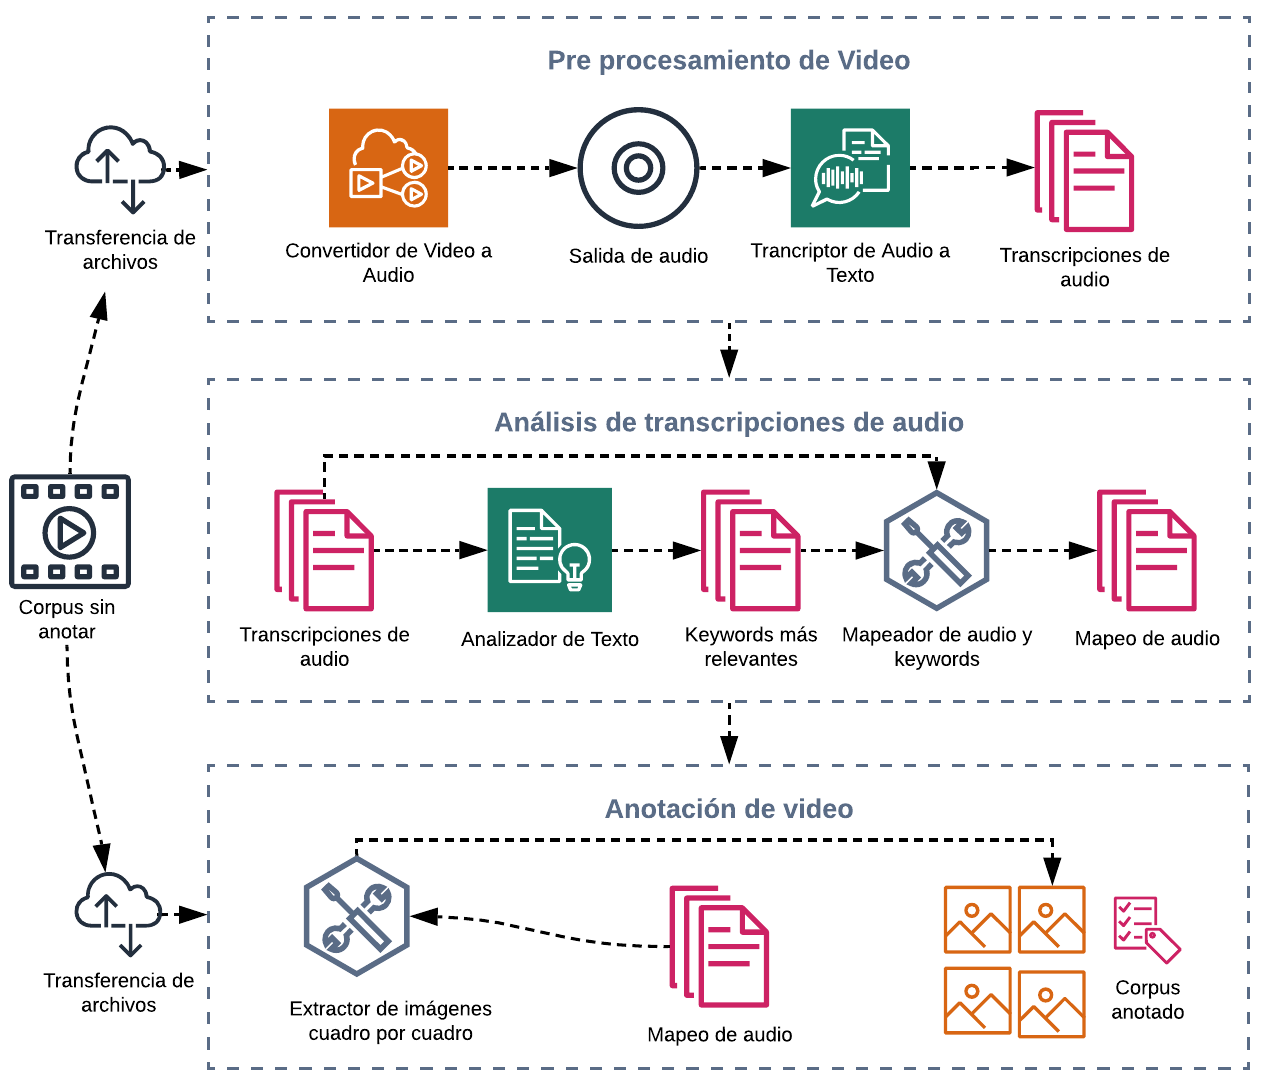
\includegraphics[width=\linewidth]{video-annotation-pipeline.png}
\caption{Video annotation process}
\end{figure}
\section{Conclusion}\label{conclusion}

\bibliographystyle{ieeetr}
\bibliography{References}


\end{document}
